\renewcommand{\theequation}{\theenumi}

\begin{enumerate}[label=\arabic*.,ref=\thesubsection.\theenumi]
\numberwithin{equation}{enumi}
\item
Find the {\em orthocentre} of  $\triangle ABC$.
\\
\solution The following code finds the required point using \eqref{eq:alt_ap} and \eqref{eq:alt_bq}
.
\begin{lstlisting}
codes/2d/orthocentre.py
\end{lstlisting}

\item Find $\vec{P}$, the foot of the altitude from $\vec{A}$ upon BC.
%
\\
\solution 
\begin{lstlisting}
codes/2d/alt_foot.py
\end{lstlisting}
\item Find $\vec{Q}$ and $\vec{R}$.
\item Draw $AP, BQ$ and $CR$ and verify that they meet at a point 
$\vec{H}$.  
\\
\solution The following code plots the altitudes in Fig. \ref{fig:alt_triangle}
\begin{lstlisting}
codes/2d/alt_draw.py
\end{lstlisting}
\begin{figure}
\centering
\includegraphics[width=\columnwidth]{./line/figs/alt_triangle.eps}
\caption{}
\label{fig:alt_triangle}
\end{figure}
\item
Find the coordinates of $\vec{D}, \vec{E}$ and $\vec{F}$ of the mid points of $AB, BC$ and $CA$ respectively 
for  $\Delta ABC$. 
\item
Find the equations of $AD,BE$ and $CF$. 
%
\item
\label{prob:median}
Find the point of intersection of $AD$ and $CF$.
\item
Verify that $\vec{O}$ is the point of intersection of $BE,CF$ as 
well.
%as
\item
Graphically show that the medians of $\Delta ABC$ meet at the centroid.
\end{enumerate}

